\section{Ordinary Least Squares (OLS)}
\subsection{Theory}
Ordinary Least Squares solves a linear, overconstrained system of equations by minimizing the squared residuals of each observation equation.
\[
min \sum_{i}^{n} v_i^2
\]

\subsection{Assumptions}
\begin{itemize}
	\item No Outliers/Blunders OLS is not robust to outliers (consider RANSAC/Robust Weighting if outliers)
	\item System of equations is linear (eg. derivative wrt each unknown is not a function of any of the unknowns)
	\item System is over-contrained (eg. Number of Observation Equations > Number of Unknowns)
	\item Error only in dependent variable (eg. mx+b = y + v $\rightarrow$ error only in y dimension)
\end{itemize}
\subsection{Equations}
\[
AX=L+V 
\]
\[
m = \text{number of observations} \hspace{1cm} 
n = \text{number of unknowns}
\]
\[
dof = \text{degrees of freedom (\# of redundant observations)} = m-n
\]
\[
A = \begin{bmatrix}
a_{11} & a_{12} & \dots & a_{1n} \\
a_{21} & a_{22} & \dots & a_{1n} \\
\vdots & \vdots & \vdots& \vdots \\
a_{m1} & a_{m2} & \dots & a_{mn} \\
\end{bmatrix}
\hspace{1cm}
X = 
\begin{bmatrix}
x_1 \\ x_2 \\ \vdots \\ x_n
\end{bmatrix}
\hspace{1cm}
L = 
\begin{bmatrix}
l_1 \\ l_2 \\ \vdots \\ l_m
\end{bmatrix}
\hspace{1cm}
V = 
\begin{bmatrix}
v_1 \\ v_2 \\ \vdots \\ v_m
\end{bmatrix}
\]
\begin{align*}
\text{Unknowns} &= \hat{X} = inv(A^TA)A^TL\\
\text{Residuals} &= V = AX - L\\
\text{Reference Variance} &= S_0^2 = \dfrac{V'V}{dof} \\
\text{Cofactor Matrix} &= Q_{xx} = inv(A^TA) \\
\text{Covariance Matrix of Unkowns} &= \Sigma_{xx} = S_0^2 Q_{xx} \\
\text{Covariance Matrix of Observations} &= \Sigma_{\hat{l}\hat{l}} = A \Sigma_{xx} A^T \\
\text{Standard Deviation of Solved Unknowns} &= \sigma_{\hat{X}} = \sqrt{diag(\Sigma_{xx})} \\
\text{Predicted L} &= \hat{L} = AX \\
\text{R$^2$ (model skill)} &= \dfrac{var(\hat{L})}{var(L)} \\
\text{RMSE } &= \sqrt{\dfrac{V^TV}{m}} \\
\end{align*}
\clearpage
\subsection{Sample Problem}
Given the points: 
\[
x = [0,1,2,3,4] \hspace{1cm} y = [5,1,7,13,24]
\]
Fit a parabola given the observation equation:
\[
y = a x^2 +b x + c
\]
Note that the observation equation is linear. The $x^2$ term is a constant once observation values are substituted.
\[
A = \begin{bmatrix}
x_1^2 & x_1 & 1 \\
x_2^2 & x_2 & 1 \\
x_3^2 & x_3 & 1 \\
x_4^2 & x_4 & 1 \\
x_5^2 & x_5 & 1 \\
\end{bmatrix} =
\begin{bmatrix}
0 & 0 & 1 \\
1 & 1 & 1 \\
4 & 2 & 1 \\
9 & 3 & 1 \\
16 & 4 & 1 \\
\end{bmatrix}
\hspace{1cm}
X = 
\begin{bmatrix}
a \\ b \\ c 
\end{bmatrix}
\hspace{1cm}
L =
\begin{bmatrix}
y_1 \\ y_2 \\ y_3 \\ y_4 \\ y_5
\end{bmatrix} = 
\begin{bmatrix}
5 \\ 1 \\ 7 \\ 13 \\ 24
\end{bmatrix}
\]
Use the Equations and solve:
\begin{table}[H]
\centering
\begin{tabular}{|c|c|c|}
\toprule
$n = 3$& %NEWCOLUMN
$m = 5$& %NEWCOLUMN
$dof = 2$\\ %NEWROW
\midrule
$\hat{X} = $$
 \begin{bmatrix}
2.14\\
-3.57\\
4.29\\
\end{bmatrix}
$
& %NEWCOLUMN
$V = $ $
 \begin{bmatrix}
-0.71\\
1.86\\
-1.29\\
-0.14\\
0.29\\
\end{bmatrix}
$
& %NEWCOLUMN
$S_0^2 = 2.86$ \\ %NEWROW
\midrule
$\Sigma_{xx} = $ $
 \begin{bmatrix}
0.20&-0.82&0.41\\
-0.82&3.55&-2.20\\
0.41&-2.20&2.53\\
\end{bmatrix}
$
& %NEWCOLUMN
$\sigma_{\hat{X}} = $ $
 \begin{bmatrix}
0.45\\
1.88\\
1.59\\
\end{bmatrix}
$
& %NEWCOLUMN
$\Sigma_{\hat{l}\hat{l}} = $ $
 \begin{bmatrix}
2.53&0.73&-0.24&-0.41&0.24\\
0.73&1.06&0.98&0.49&-0.41\\
-0.24&0.98&1.39&0.98&-0.24\\
-0.41&0.49&0.98&1.06&0.73\\
0.24&-0.41&-0.24&0.73&2.53\\
\end{bmatrix}
$
\\ %NEWROW
\midrule
$Q_{xx} = $ $
 \begin{bmatrix}
0.07&-0.29&0.14\\
-0.29&1.24&-0.77\\
0.14&-0.77&0.89\\
\end{bmatrix}
$
& %NEWCOLUMN
$\hat{L} = $$
 \begin{bmatrix}
4.29\\
2.86\\
5.71\\
12.86\\
24.29\\
\end{bmatrix}
$
& %NEWCOLUMN
$R^2 = 0.9821$ \hspace{1cm} $RMSE = 1.07$\\ %NEWROW
\bottomrule
\end{tabular}
\end{table}


\begin{figure}[H]
	\centering
	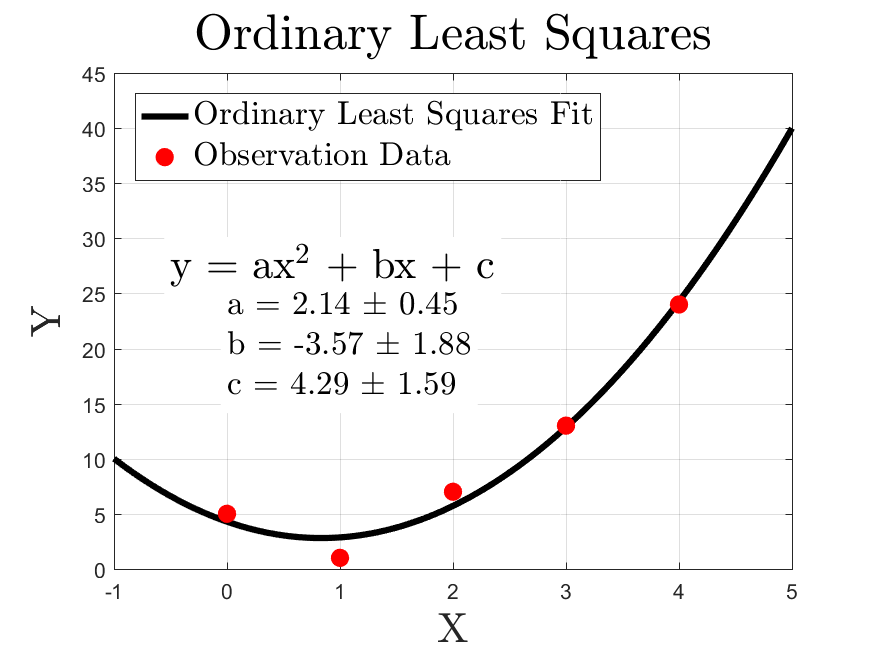
\includegraphics[height = 3.25in]{OLSexample.png}
\end{figure}

\subsection{Example Matlab Code}
\lstinputlisting[
label      = {alg:exampleOLS},
caption    = {exampleOLS.m},
style      = Matlab-editor,
basicstyle = \mlttfamily,
firstline  = 1,
lastline   = 24,
firstnumber= 1
]{exampleOLS.m}

\lstinputlisting[
label      = {alg:exampleOLS2},
caption    = {The Matlab built in function LSCOV generates the same results},
style      = Matlab-editor,
basicstyle = \mlttfamily,
firstline  = 25,
lastline   = 26,
firstnumber= 25
]{exampleOLS.m}